%------------------------------------------------------------------------------%

\subsubsection{Contexto}

\begin{frame}{Origem}
  O \textbf{Minimum Scan Cover} (MSC) foi introduzido em 2021~\cite{Fe21} como um problema de comunicação ponto a ponto entre satélites:
  \bigbreak
  \begin{minipage}{\linewidth}
    \centering
    \only<1>{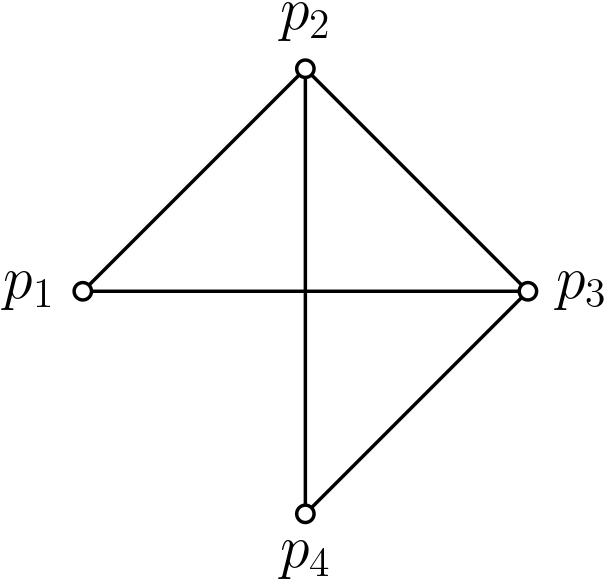
\includegraphics[height=5cm]{MSC/instance/Temp-0.png}}%
    \only<2>{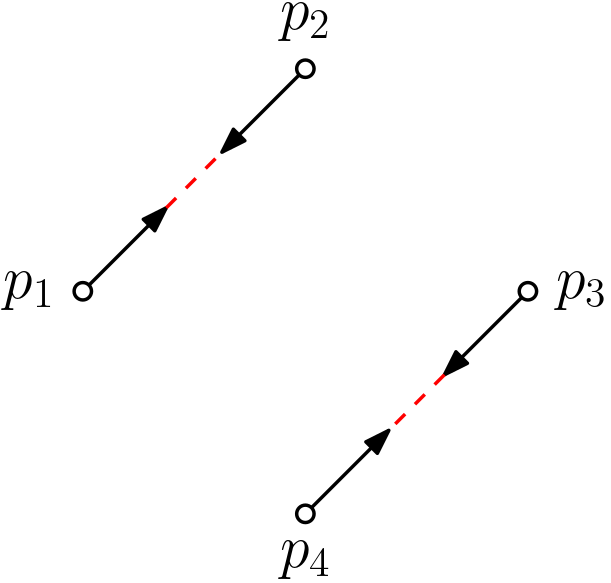
\includegraphics[height=5cm]{MSC/instance/Temp-1.png}}%
    \only<3>{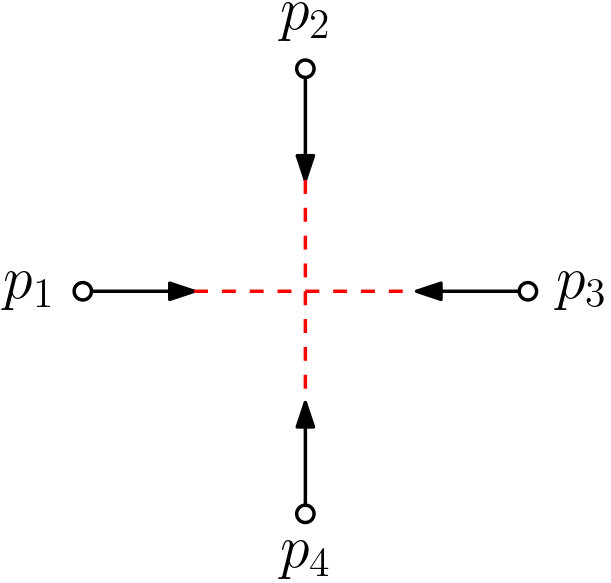
\includegraphics[height=5cm]{MSC/instance/Temp-2.png}}%
    \only<4>{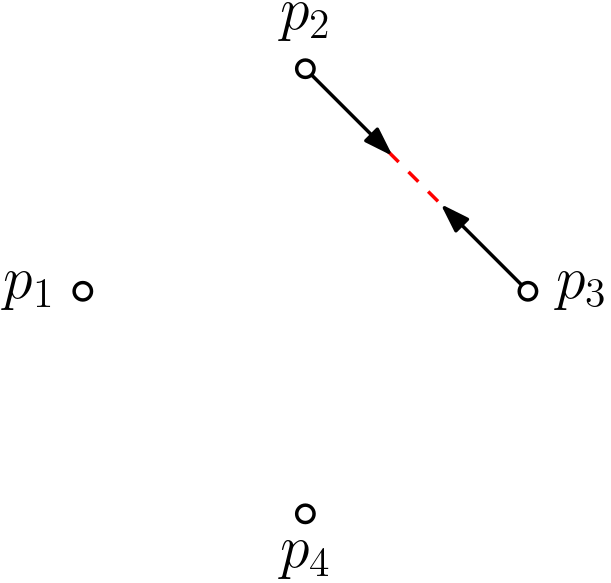
\includegraphics[height=5cm]{MSC/instance/Temp-3.png}}%
  \end{minipage}
\end{frame}

\begin{frame}{Motivação}
  \begin{itemize}[<+->]

    \item É possível usar tanto transmissão direcional quanto recepção omnidirecional;

    \item Mas exige duas antenas, aumentando custo e complexidade.

  \end{itemize}
\end{frame}

\begin{frame}{Definição - Instância}
  \begin{itemize}[<+->]

    \item Conjunto $P = \{p_1, \dots, p_n\}\subseteq \R^d$ de posições distintas;

    \item Grafo $G=(P, E)$ onde $E\subseteq P\times P$.

  \end{itemize}
\end{frame}

\begin{frame}{Definição - Solução}
  \textbf{Escalonamento} ${\cals\colon E\to \R^+}$ onde queremos minimizar $\max\limits_{e \in E} \cals(e)$:
  \begin{minipage}{\linewidth}
    \centering
    \vspace*{1cm}
    \only<1>{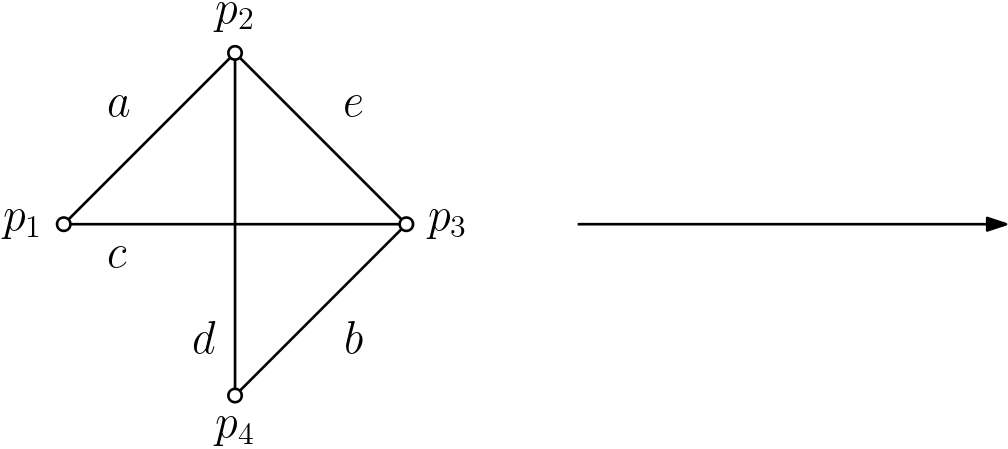
\includegraphics[height=4cm]{MSC/solution/Sol-0.png}}%
    \only<2>{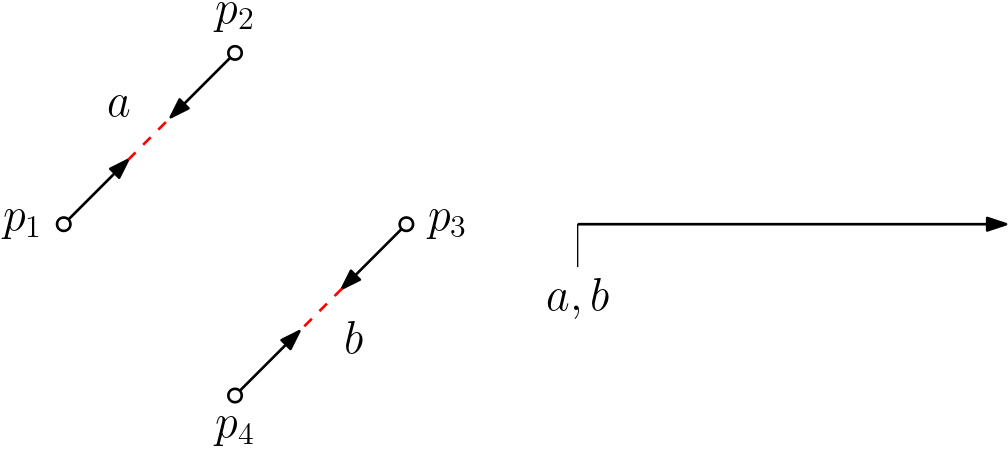
\includegraphics[height=4cm]{MSC/solution/Sol-1.png}}%
    \only<3>{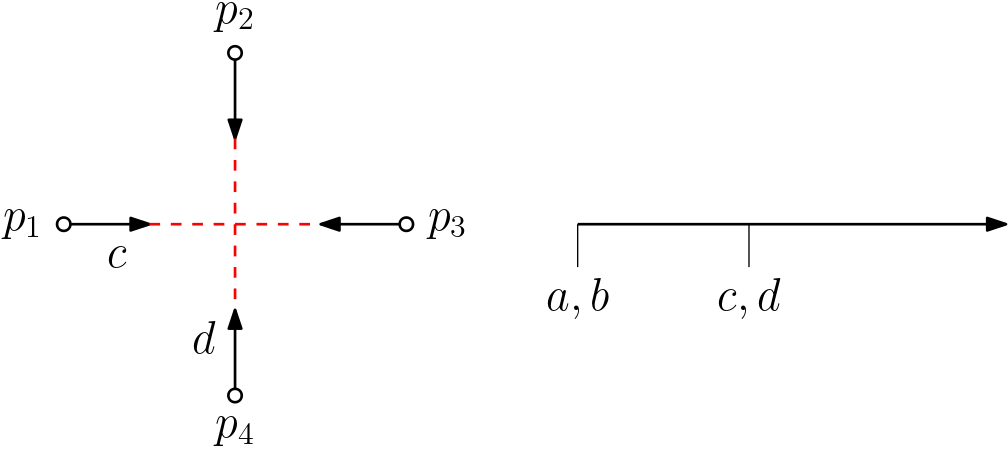
\includegraphics[height=4cm]{MSC/solution/Sol-2.png}}%
    \only<4>{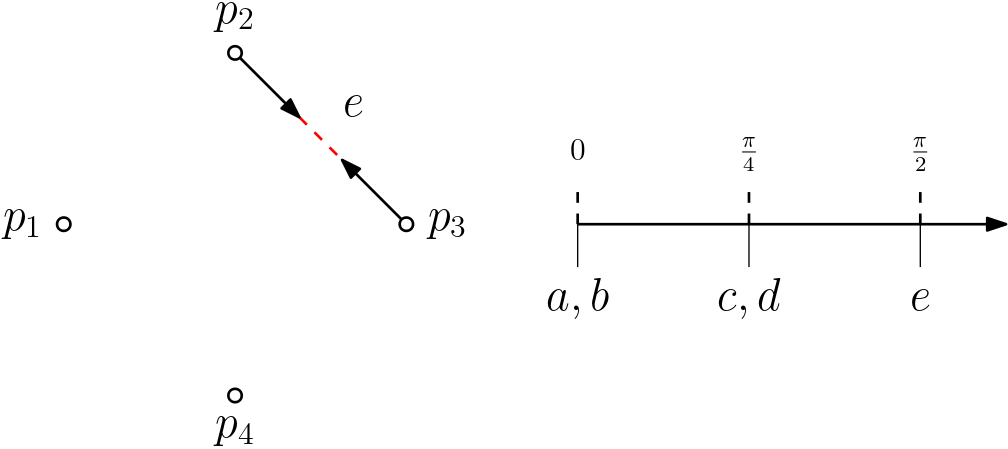
\includegraphics[height=4cm]{MSC/solution/Sol-3.png}\bigbreak}
    \only<4>{$\cals(a)=\cals(b)=0$, $\cals(c)=\cals(d)=\frac{\pi}{4}$ e $\cals(e)=\frac{\pi}{2}$}
  \end{minipage}
\end{frame}

%------------------------------------------------------------------------------%

\subsubsection{Resultados Teóricos para 1D}

\begin{frame}{Resultado Anterior}
  \begin{thm}[Fekete et al.~\cite{Fe21}]
    Mesmo em 1D, para todo $\gamma \geq 1$, uma $\gamma$-aproximação para o MSC implica que $P = NP$.
  \end{thm}
\end{frame}

\begin{frame}{Nossos Resultados}
  \setbeamercolor{block body}{bg=green!35!white}
  \begin{thm}
    Existe um algoritmo \FPT para o MSC em 1D, parametrizado pela largura de árvore $k$, que roda em tempo $k^{O(k)} \cdot n$.
  \end{thm}

  \pause
  \begin{cor}
    Existe uma $3$-aproximação para o MSC em 1D em grafos planares, que roda em tempo $O(n^2)$.
  \end{cor}
\end{frame}

%------------------------------------------------------------------------------%

\subsubsection{Resultados Teóricos para 2D}

\begin{frame}{Resultados Anteriores}
  \begin{thm}[Fekete et al.~\cite{Fe21}]
    Mesmo em 2D, para todo $\gamma < \nicefrac{3}{2}$, uma $\gamma$-aproximação para o MSC em grafos bipartidos implica que $P = NP$.
  \end{thm}

  \pause
  \begin{thm}[Fekete et al.~\cite{Fe21}]
    Existe uma $\frac{9}{2}$-aproximação para o MSC em 2D em grafos bipartidos.
  \end{thm}
\end{frame}

\begin{frame}{Preliminares}
  \centering
  Uma instância usando $\ell=8$ direções:

  \bigskip
  \begin{minipage}{\linewidth}
    \centering
    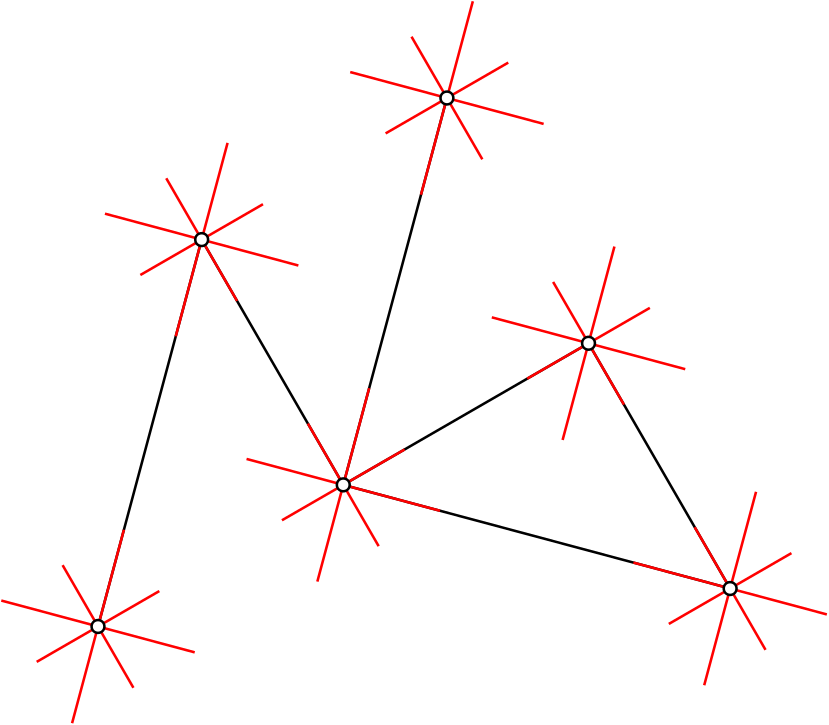
\includegraphics[height=5cm]{MSC/directions.png}
  \end{minipage}
\end{frame}

\begin{frame}{Nossos Resultados}
  \setbeamercolor{block body}{bg=green!35!white}
  \begin{thm}
    Existe um algoritmo \FPT para MSC em 2D, parametrizado pela largura de árvore $k$ e $\ell$, que roda em tempo $k^{O(k \ell \log(\ell))} \cdot n$.
  \end{thm}

  \pause
  \begin{cor}
    Existe uma $3$-aproximação para MSC em 2D em grafos planares parametrizada por $\ell$, que roda em tempo $\ell^{O(\ell)} \cdot n + O(n^2)$.
  \end{cor}
\end{frame}

\begin{frame}{Preliminares}
  \centering
  Uma instância de ângulo mínimo não nulo $\lambda$:

  \bigskip
  \begin{minipage}{\linewidth}
    \centering
    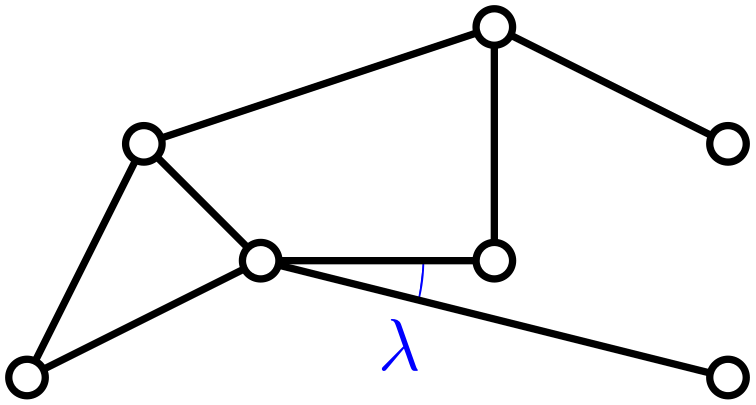
\includegraphics[height=2.5cm]{MSC/lambda.png}
  \end{minipage}
\end{frame}

\begin{frame}{Nosso Resultado}
  \setbeamercolor{block body}{bg=green!35!white}
  \begin{thm}
    Existe uma $2$-aproximação para o MSC em 2D parametrizada pela largura de árvore $k$ e $\lceil \nicefrac{1}{\lambda} \rceil$, que roda em tempo $\lambda^{-O(k^2 + \frac{k \log k}{\lambda})} \cdot (\log k)^{O(k^2)} \cdot n$.
  \end{thm}
\end{frame}

\begin{frame}{Esboço da Prova}
    \begin{itemize}[<+->]
        \item Seja $\cali = (P, G)$ uma instância de ângulo mínimo não nulo $\lambda$;

        \item Recebemos uma decomposição em árvore de $G$ com largura $k$;

        \item \emph{WLOG}, considere que $\lambda < \pi$.
    \end{itemize}
\end{frame}

\begin{frame}{}
    \begin{itemize}[<+->]
        \item Seja $M := \floor{\nicefrac{\pi}{\lambda}} \geq 1$;

        \item O disco ao redor de cada $p_i\in P$ é dividido em $4M$ \textbf{setores}:
    \end{itemize}
    
    \bigskip
    \pause
    \begin{minipage}{\linewidth}
        \centering
        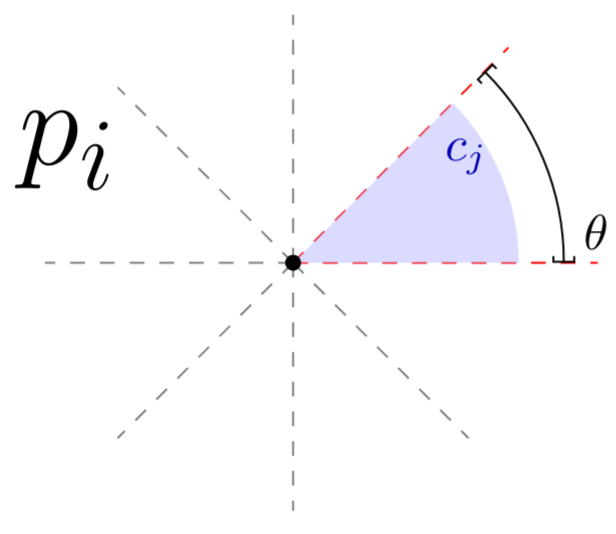
\includegraphics[height=4cm]{MSC/angle.png}
    \end{minipage}

    \bigskip
    \centering
    $\theta := \frac{\pi}{2M} < \lambda$ e os setores são $c_j$ para $j \in \{0, \dots, 4M-1 \}=[4M-1]$
\end{frame}

\begin{frame}{}
    Consideramos uma relaxação ${\hat \cali:= \cali}$ dependendo de $\theta$:
    
    \bigskip
    \pause
    \begin{minipage}{\linewidth}
        \centering
        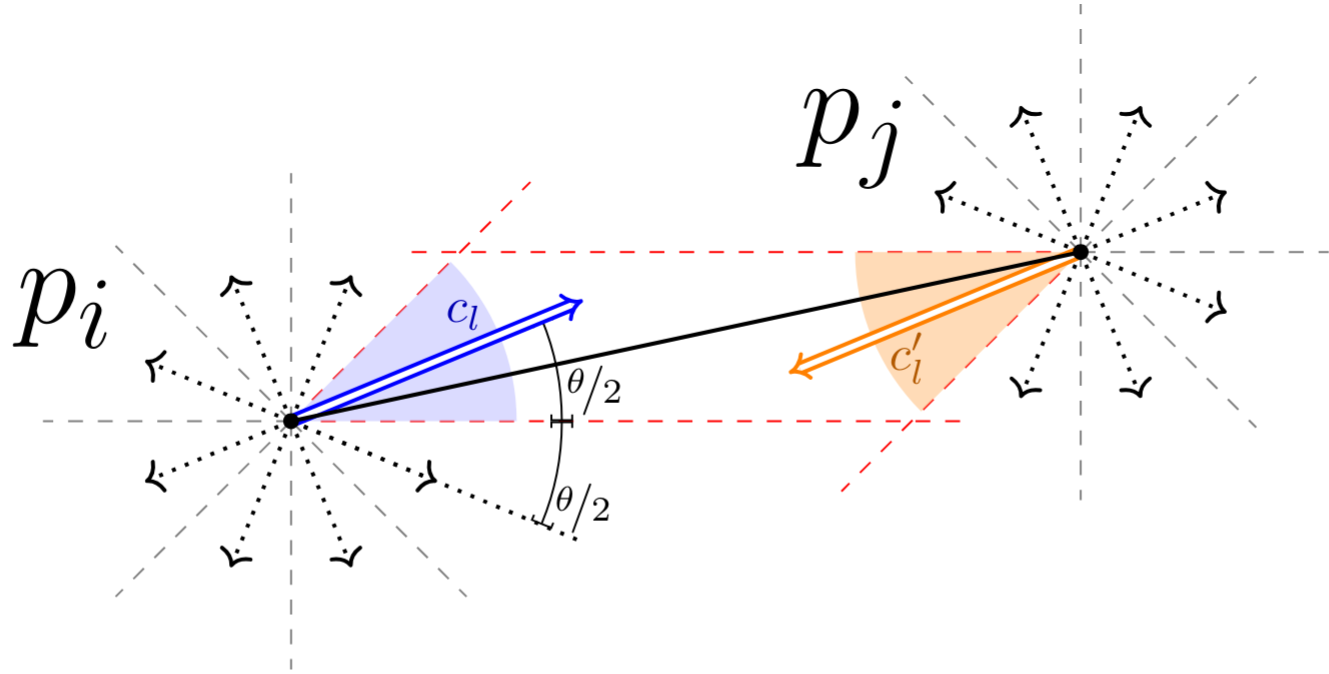
\includegraphics[height=5cm]{MSC/discrete.png}
    \end{minipage}
\end{frame}

\begin{frame}{}
    \begin{obs}
        Cada solução ótima de custo $N \theta$ corresponde a uma função \mbox{$\hat h\colon P \to [4M-1]^{N+1}$}.
    \end{obs}
\end{frame}

\begin{frame}{}
    \begin{obs}
        \label{obs:msc2d}
        Seja $t^*$ o ótimo de $\cali$. Então, $t^* \leq 3\pi\ceil{\log_2(k+1)}$
    \end{obs}
\end{frame}

\begin{frame}{}
    Pela \ref{obs:msc2d}ª Observação, existe uma solução de $\hat \cali$ com custo $N \theta$, onde:

    \bigskip
    \centering
    $N \leq \frac{3\pi\ceil{\log_2(k+1)}}{\theta} = 6\floor{\nicefrac{\pi}{\lambda}} \ceil{\log_2(k+1)}$
\end{frame}

\begin{frame}{}
    \centering
    Particionamos o intervalo de tempo $[0,\ (N+1) \theta)$:

    \pause
    \vspace*{2cm}
    \begin{minipage}{\linewidth}
        \centering
        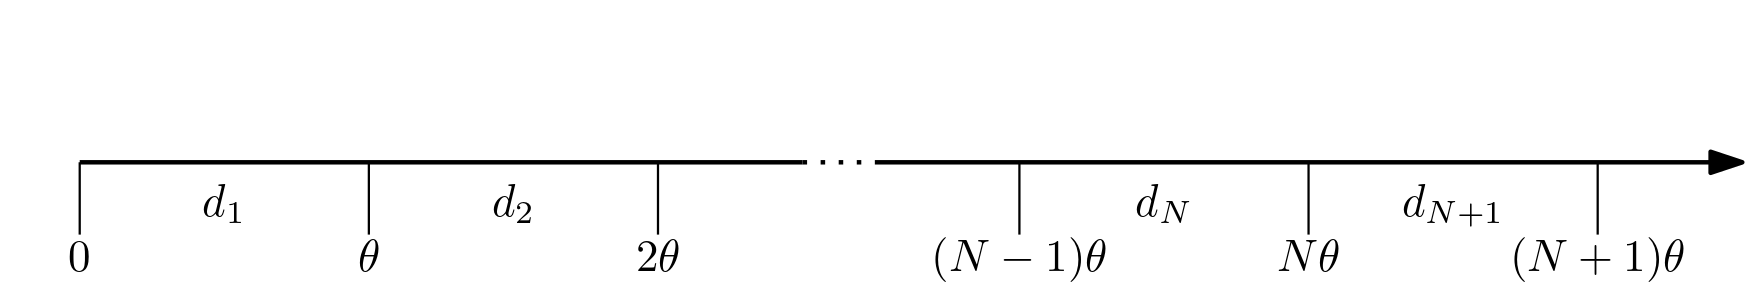
\includegraphics[width=10cm]{MSC/interval.png}
    \end{minipage}
\end{frame}

\begin{frame}{}
    \only<1>{\begin{lem}
        \label{lemma:1}
        Existe uma solução de custo no máximo $\floor{\nicefrac{t^*}{\theta}} \theta$ para $\hat \cali$, que mapeia arestas para pontos em $\{i\cdot \theta\ |\ i \in [N]\}$.
    \end{lem}}

    \centering 
    \only<2>{Seja {\color{blue} $\cals^*$} uma solução ótima para $\cali$.}
    \only<3,4>{Se o ângulo entre $\mathbf{e}$ e $\mathbf{f}$ não é zero, então ele é ao menos $\lambda>\theta$:}
    \only<5>{Caso contrário, o ângulo entre $\mathbf{e}$ e $\mathbf{f}$ é zero:}

    \begin{minipage}{\linewidth}
        \vspace*{2cm}
        \centering
        \only<4>{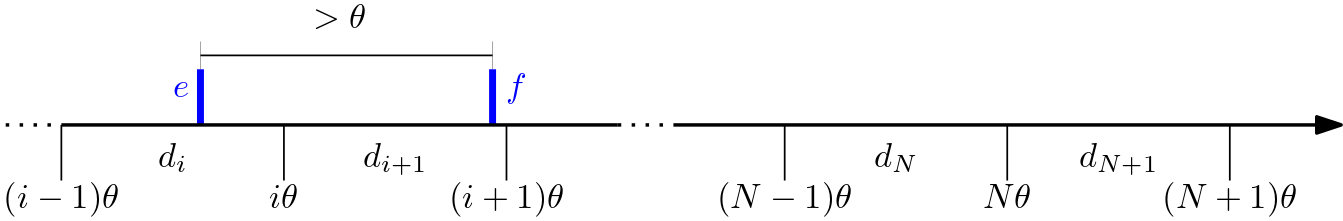
\includegraphics[width=10cm]{MSC/lemma/lema_1.png}}%
        \only<5>{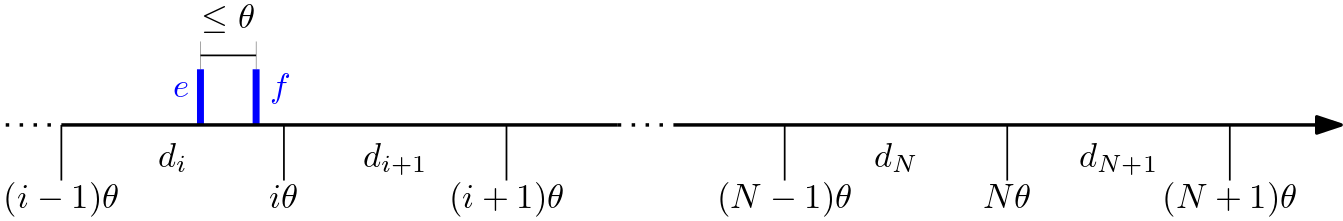
\includegraphics[width=10cm]{MSC/lemma/lema_2.png}}%
    \end{minipage}
\end{frame}

\begin{frame}{}
    \centering
    Construímos uma solução {\color{red} $\hat \cals$} para $\hat \cali$ a partir de {\color{blue} $\cals^*$}:

    \begin{minipage}{\linewidth}
        \vspace*{2cm}
        \centering
        \only<2>{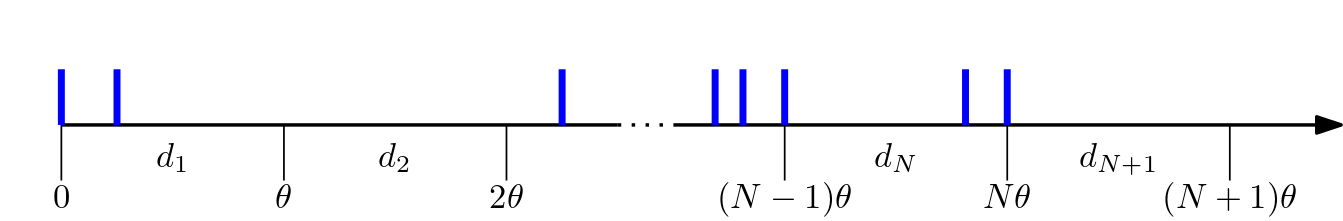
\includegraphics[width=10cm]{MSC/lemma/lema_3.png} \hfill{}\\\phantom{\qed}}%
        \only<3>{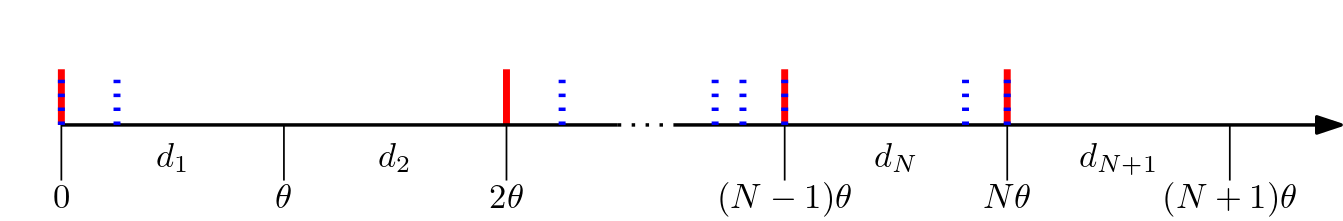
\includegraphics[width=10cm]{MSC/lemma/lema_4.png} \hfill{}\\\qed}%
    \end{minipage}
\end{frame}

\begin{frame}{}
    Usando programação dinâmica sobre a decomposição em árvore calculamos uma solução ótima para $\hat\cali$ em tempo:

    \bigskip
    \centering
    $N^{O(k^2)}\cdot M^{O(Nk)}\cdot k^{O(1)} \cdot n = \lambda^{-O(k^2+\frac{k\log k}{\lambda})}\cdot (\log k)^{O(k^2)}\cdot n$
\end{frame}

\begin{frame}{}
    \centering
    Seja {\color{red} $\hat \cals^*$} uma solução ótima para $\hat \cali$:

    \begin{minipage}{\linewidth}
        \vspace*{2cm}
        \centering
        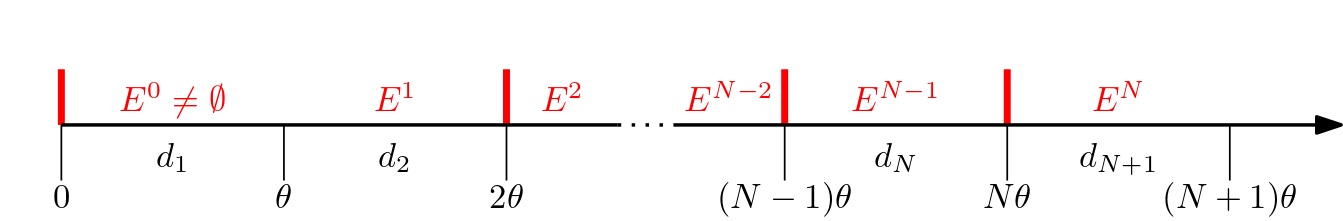
\includegraphics[width=10cm]{MSC/final/final_1.png}
    \end{minipage}
\end{frame}

\begin{frame}{}
    \centering
    \begin{itemize}[<+->]
        \item Se o ângulo entre $\mathbf{e}$ e $\mathbf{f}$ não é zero, então é maior que $\theta$;
        
        \item Logo, $|{\color{red} \hat \cals^*}(\mathbf{e})-{\color{red} \hat \cals^*}(\mathbf{f})|> \theta$, e não pertencem ao mesmo $E^i$.
    \end{itemize}
\end{frame}

\begin{frame}{}
    \centering
    Construímos uma solução {\color{blue} $\cals$} para $\cali$ a partir de {\color{red} $\hat \cals^*$}:

    \begin{minipage}{\linewidth}
        \vspace*{2cm}
        \centering
        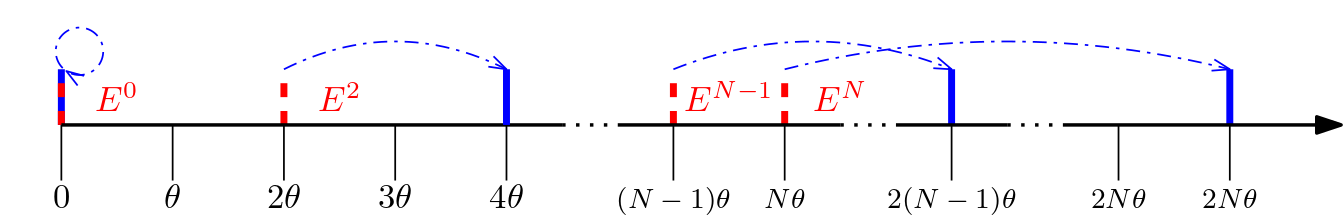
\includegraphics[width=10cm]{MSC/final/final_2.png}
    \end{minipage}
\end{frame}

\begin{frame}{}
    \centering
    \only<1>{Arestas no mesmo $E^i$ \checkmark}
    \only<2-6>{$\mathbf{e} \in E^i$ e $\mathbf{f} \in E^j$ onde $i\ne j$:\\\bigskip}
    \only<5>{\centering Sabemos que $|{\color{red} \hat \cals^*}(e) - {\color{red} \hat \cals^*}(f)|=|i-j|\cdot \theta \ge \phi$}
    \only<6>{\centering Logo, por definição, $|{\color{blue} \cals}(e) - {\color{blue} \cals}(f)| = 2|i-j| \cdot \theta \ge \phi + \theta$}

    \begin{minipage}{\linewidth}
        \vspace*{0.5cm}
        \centering
        \only<2>{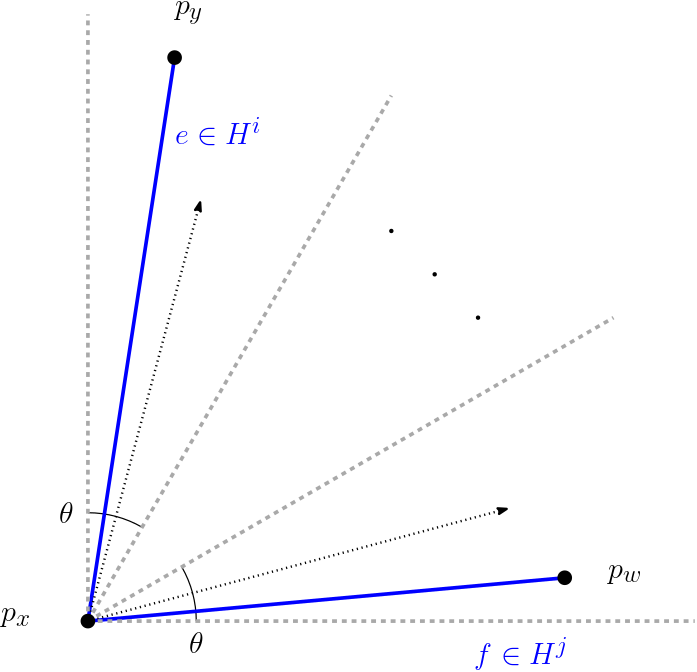
\includegraphics[height=6cm]{MSC/end/end_2.png}}%
        \only<3>{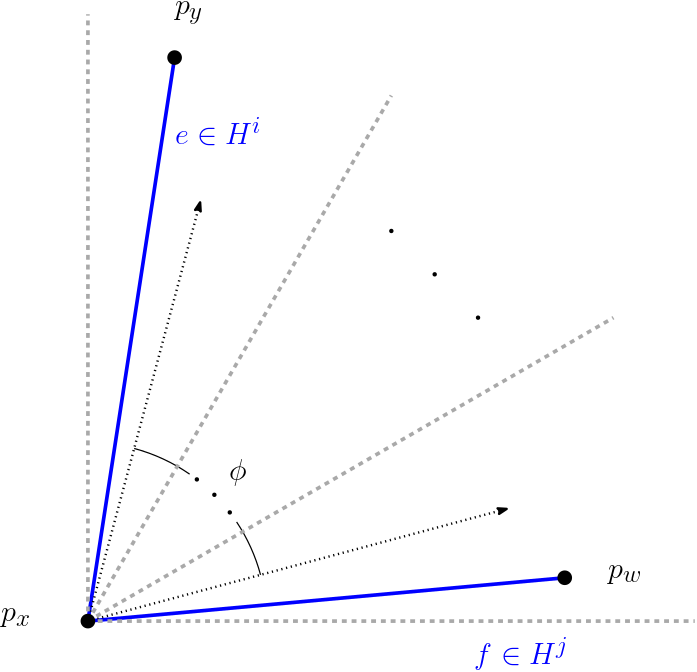
\includegraphics[height=6cm]{MSC/end/end_3.png}}%
        \only<4-6>{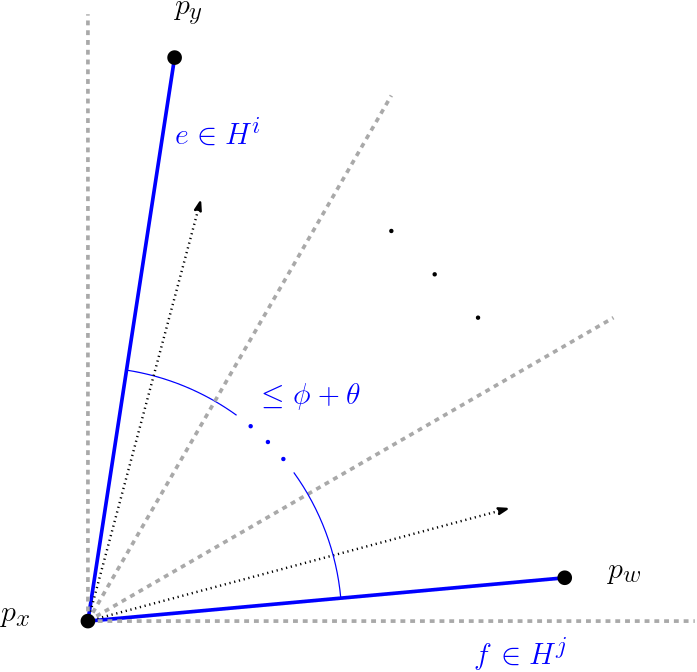
\includegraphics[height=6cm]{MSC/end/end_4.png}}%
    \end{minipage}
\end{frame}

\begin{frame}{}
    \centering
    Arestas no mesmo $E^i$ \checkmark\\\bigskip
    $\mathbf{e} \in E^i$ e $\mathbf{f} \in E^j$ onde $i\ne j$ \checkmark\\\bigskip
    Então, ${\color{blue} \cals}$ é válido.
\end{frame}

\begin{frame}{}
    \centering
    Portanto, pelo \ref{lemma:1}º Lema, o custo de ${\color{blue} \cals}$ é no máximo $2\floor{\nicefrac{t^*}{\theta}}\theta \le 2t^*$ \\\qed
\end{frame}

\begin{frame}{Nosso Resultado}
  \setbeamercolor{block body}{bg=green!35!white}
  \begin{cor}
    Existe uma $5$-aproximação para o MSC em 2D em grafos planares parametrizada por $\lceil \nicefrac{1}{\lambda} \rceil$, que roda em tempo $\lambda^{-O(\nicefrac{1}{\lambda})} \cdot n + O(n^2)$.
  \end{cor}
\end{frame}
